% Created 2021-05-09 dim. 15:33
% Intended LaTeX compiler: pdflatex
\documentclass[11pt, letterpaper]{article}
         \usepackage[document]{ragged2e}
\usepackage[utf8]{inputenc}
\usepackage[T1]{fontenc}
\usepackage{graphicx}
\usepackage{grffile}
\usepackage{longtable}
\usepackage{wrapfig}
\usepackage{rotating}
\usepackage[normalem]{ulem}
\usepackage{amsmath}
\usepackage{textcomp}
\usepackage{amssymb}
\usepackage{capt-of}
\usepackage{hyperref}
\author{Groupe 7: Hery ANDRIANANTENAINA, Nicolas BOUTON, Ali LAKBAL}
\date{Mai 2021}
\title{Rapport du Second Semestre sur le support de la Vectorisation et de la Parallèlisation dans Verificarlo}
\hypersetup{
 pdfauthor={Groupe 7: Hery ANDRIANANTENAINA, Nicolas BOUTON, Ali LAKBAL},
 pdftitle={Rapport du Second Semestre sur le support de la Vectorisation et de la Parallèlisation dans Verificarlo},
 pdfkeywords={},
 pdfsubject={},
 pdfcreator={Emacs 27.2 (Org mode 9.4.4)}, 
 pdflang={English}}
\begin{document}

\maketitle
\tableofcontents


\section{Introduction}
\label{sec:org73549da}

Ce rapport fait suite au précédent. Les informations rédigées sur le précédent
rapport doivent donc être comprises afin de pouvoir comprendre la suite du
rapport.

Nous rappelons tout de même qu'il faut configurer \textbf{verificarlo} avec \textbf{clang}
car nous utilisons les types vectoriels qu'il propose afin d'éviter les
intrinsèques qui seraient dépendantes de l'architecture. (réf: \hyperref[orgb824849]{2})

Les sources sont toujours disponibles sur notre organisation Github:

\url{https://github.com/Safecarlo}

Notamment les sources pour le support de la vectorisation qui se trouvent sur
la branche \textbf{vectorisation} de notre fork:

\url{https://github.com/Safecarlo/verificarlo/tree/vectorization}

Un autre répertoire important est celui du benchmark que nous avons utilisé
pour évaluer l'efficacité de notre implémentation vectorielle:

\url{https://github.com/Safecarlo/benchmark}

Un dernier répertoire qui affiche les flottants simple et double précision
sous différents formats:

\url{https://github.com/Safecarlo/print\_floating\_point}

\section{Partage des tâches}
\label{sec:orgee78af0}

Ce semestre nous avons décidé de répartir les tâches de la façon suivante:
\begin{itemize}
\item Nicolas sur le support de la Vectorisation
\item Hery et Ali sur le support de la Parallélisation
\end{itemize}

\section{Support de la vectorisation}
\label{sec:org9031b1b}
\subsection{Point git}
\label{sec:orgdd333d7}
\subsubsection{Rebasage}
\label{sec:org491a855}

Durant le semestre, des modifications ont été apportées sur la branche master
du répertoire public \textbf{verificarlo} qui est disponible sur la forge
\textbf{Github}. Pour ne pas être trop éloigné de la version scalaire de
cette branche nous avons donc décidé de rapatrier les modifications de la
branche master de \textbf{verificarlo} vers notre branche master de notre fork
\textbf{Safecarlo}.

Le problème étant que nous avons utilisé la stratégie par fusion (qui était
par défaut) qui tri les modifications (commits) des deux branches (celle
de verificarlo et la notre dans Safecarlo) par date.

Nous avons donc constaté que ce n'était pas la meilleure version pour
rapatrier les modifications (commits) car ils se retrouvaient mélangés avec
les nôtres.

Nous aurions pu et dû utiliser la stratégie par rebasage afin de grouper les
modifications de la branche master de \textbf{verificarlo} à la fin de nos
modifications (commits) pour éviter de les éparpiller dans nos modifications
(commits).

\subsubsection{Pull requests sur verificarlo}
\label{sec:orgcbd01fa}

Des pull requests ont été fait sur verificarlo, notamment pour nettoyer le
répertoire de tests qui n'était pas nettoyer par la cible "clean" du
makefile. Comme verificarlo utilise les \textbf{autotools}, la cible n'est pas
directement disponible et nous avons dû utiliser une dépendance de la cible
"clean" des \textbf{autotools} qui est "clean-local". Et avec cette cible nous
appelons notre cible, qui nettoie le répertoire \texttt{tests/}, en la mettant
comme dépendance de la cible "clean-local".

Nous avons fait cette PR (pull requests) car nous développions des tests
dans notre fork de verificarlo afin de s'assurer que nos changement dans le
code soit bon. Le problème était que de multiples fichiers était créés mais
j'avais supprimés. Et cela était un peu embêtant lorsque nous voulions
lister nos fichier (avec la commande ls) ou bien utiliser un script car les
anciens résultats n'étaient pas effacés. Donc nous les enlevions
manuellement au début puis nous avons vite arrêté. De plus il y avait 2
fichiers qui était créer à la configuration de verificarlo dans le
répertoire qui n'était pas non plus nettoyé.

Tous ces fichiers non nettoyés nous embêtaient pour utiliser git car nous
éditions aussi d'autre fichier et nous avions les 2 fichiers créer par la
configuration qui apparaissaient dans la liste des fichiers possible à
indexer (\texttt{git status}).

\subsection{Mise à jour du backend \textbf{ieee}}
\label{sec:orgb95dd98}
\subsubsection{Ajout du compte des opérations flottantes vectorielles dans le backend \textbf{ieee}}
\label{sec:orgf47144b}

Lors de la mise à jour de notre branche master, nous nous sommes rendus
comptes que des changements ont été apportés au backend \textbf{ieee}. Notamment
celle du comptage des opérations. Cependant le comptage des opérations
flottante ne comptait que les opérations scalaire comme ci-dessous:

\begin{verbatim}
operations count:
     mul = 1 total count;
     div = 0 total count;
     add = 0 total count;
     sub = 0 total count;
\end{verbatim}

Nous avons donc ajouté le compte spécifiques de chaque opérations
vectorielles et décidé d'afficher un pourcentage de vectorisation.

\begin{verbatim}
operations count:
     mul = 1 total count; 100.00% vectorized;
     div = 0 total count;   0.00% vectorized;
     add = 0 total count;   0.00% vectorized;
     sub = 0 total count;   0.00% vectorized;
\end{verbatim}

Cependant, l'affichage ne nous semblait pas suffisant car nous avions
l'information du nombre de chaque opérations flottantes par taille mais nous
ne l'utilisions pas. Nous avons donc rajouté le pourcentage pour chaque
taille de vecteur.

\begin{verbatim}
operations count:
     mul = 1 total count; 100.00% vectorized;   0.00% 2x; 100.00% 4x;   0.00% 8x;   0.00% 16x
     div = 0 total count;   0.00% vectorized;   0.00% 2x;   0.00% 4x;   0.00% 8x;   0.00% 16x
     add = 0 total count;   0.00% vectorized;   0.00% 2x;   0.00% 4x;   0.00% 8x;   0.00% 16x
     sub = 0 total count;   0.00% vectorized;   0.00% 2x;   0.00% 4x;   0.00% 8x;   0.00% 16x
\end{verbatim}

Comme vous pouvez le constatez, la ligne afficher est très grandes, et il
arrive que l'on veuille séparer notre écran en 2 (pour x ou y raison) et que
l'affichage est environ restreint à 80 caractères. C'est pourquoi nous avons
fait un affichage en 2 lignes:

\begin{verbatim}
operations count:
     mul = 1 total count; 100.00% vectorized;
           by size:   0.00% 2x; 100.00% 4x;   0.00% 8x;   0.00% 16x
     div = 0 total count;   0.00% vectorized;
           by size:   0.00% 2x;   0.00% 4x;   0.00% 8x;   0.00% 16x
     add = 0 total count;   0.00% vectorized;
           by size:   0.00% 2x;   0.00% 4x;   0.00% 8x;   0.00% 16x
     sub = 0 total count;   0.00% vectorized;
           by size:   0.00% 2x;   0.00% 4x;   0.00% 8x;   0.00% 16x
\end{verbatim}

Le problème avec cette dernière version est qu'elle est moins lisible que
la précédente où toutes les informations sont alignés.

\begin{enumerate}
\item Apport de cette modification
\label{sec:org790ca8a}

Cette fonctionnalité supplémentaire pourra permettre aux utilisateurs de
pouvoir très simplement voir si leurs code est vectorisé sans passé par le
code assembleur. De plus les outils qui permettent d'évaluer le taux de
vectorisation des opérations dans un code mélangent les opérations sur les
entiers avec celles des opérations flottantes. D'où un intérêt particulier
d'utiliser cette fonctionnalité sur un code de calcul utilisant des nombres
flottants.
\end{enumerate}

\subsubsection{Tests}
\label{sec:orga9b22db}

Nous avons aussi ajouté des tests plus approfondis pour ce backend avec des
nombres aléatoirement choisis de sorte à avoir des nombres négatif, des
nombres avec un exposant négatif ou bien même des nombre avec un exposant
positif dans le même vecteur afin de s'assurer que l'implémentation
fonctionne.

\subsection{Vectorisation du backend \textbf{vprec}}
\label{sec:org73c8fa0}

Ce backend permet de gérer les cas des nombres spéciaux comme les nombres
\textbf{dénormaux} et les nombres \textbf{infinis}. Cependant ces cas restent rares dans les
codes de calculs. C'est pourquoi nous avons décidé de prioriser la
vectorisation pour les cas des nombres \textbf{normaux}.

\subsubsection{Petit rappel des cas spéciaux}
\label{sec:orged519e5}

Prenons comme exemple une précision de 3 et une portée de 2 pour un type
flottant simple précision (donc nous avons 1 bit de signe, 2 bit d'exposant
et 3 bit de pseudo-mantisse). Prenons \hyperref[org6f58747]{la formule du standard \textbf{IEEE754}} qui
est:
(-1)\^{}S * 2\^{}(E - (2\^{}(e - 1) - 1)) * (1 + P / 2\^{}p)
\begin{itemize}
\item \textbf{plus petit normal:} 0
\item \textbf{plus grand normal:} 1,75
\item \textbf{plus petit dénormal:} 0,125
\item \textbf{plus grand dénormal:} 0,875
\item \textbf{infini}: nombre supérieur à 1,75 ou inférieur à 0,125
\end{itemize}

Voir la \hyperref[orgf991456]{figure 1}.

\begin{enumerate}
\item Parenthèse sur notre mini code pour afficher les flottants sous différents formats
\label{sec:org6bc0c21}

Nous avons aussi écrit un mini code qui permet de visualiser sous différent
format les flottants simple et double précision, ce qui nous a aidé à
vérifier si nos calcul était juste pour créer cette partie et ce schéma.

\url{https://github.com/Safecarlo/print\_floating\_point}

Les résultats affichés sont sous le format \textbf{IEEE754}. Donc si on utilise
\textbf{verificarlo} avec son backend \textbf{vprec} qui nous permet de simuler une
précision custom sur les calculs, c'est pourquoi nous faisons une addition
avec \textbf{0} pour l'activer, alors le résultat peut sembler faux mais est
correct du fait que c'est une simulation et que le stockage reste sous le
format \textbf{IEEE754}.
\end{enumerate}

\subsubsection{Tests}
\label{sec:orgdcb5bfd}

Tout d'abord comme pour le premier semestre nous avons ajouté des tests pour
tester notre implémentations vectorielles des opérations vectorielles. Nous
avons choisi de faire des tests simple c'est pourquoi nous avons modifié
le test \textbf{tests\_vprec\_backend\_simple}.

Pour ce faire nous avons "copié/collé" les entrées scalaires car nous étions
sûr que ces entrées fonctionnaient. Notre code prend donc 2 lignes d'entrées car il
ne test que les vecteurs de taille 2 (c'est pourquoi il prend 2 lignes
d'entrées). La première ligne correspond au premier élément de chaque vecteur
d'entrée (a et b), et la deuxième ligne le deuxième élément de chaque
vecteur. Il garde ainsi les mêmes opérations que pour les scalaires ce qui
peut faciliter le changement d'un calcul si jamais il s'avère qu'il y en est
un qui soit mauvais.

Cependant le test ne test que la multiplication. Mais nous testons pour les
2 formats flottants du \textbf{C}, le format \textbf{simple précision} et le format
\textbf{double précision}.

Ici nous n'avons pas vraiment besoin de tester les autres tailles ainsi que
les autres opérateurs car nous avions fait au premier semestre un test qui
le faisait, certes simple mais il le faisait. De plus nous avons ajouté les
tests pour les nombres normaux mais pas pour les nombres infini car nous
avions un problème avec le retour du script qui calcul avec la librairie
\textbf{mpfr}.

\subsubsection{Structures}
\label{sec:org620bc6c}

Tout d'abord nous avons remarqué que le backend utilise des structures pour
faciliter la compréhension des calculs. Or les structures comportent des
types scalaires. Il faut donc créer de nouvelles structures pour les types
vectoriels que propose \textbf{clang}.

\begin{enumerate}
\item Code de la version scalaire pour les flottants
\label{sec:org0bfc592}

\begin{verbatim}
typedef union {

  float f32;
  uint32_t u32;
  int32_t s32;

  /* Generic fields */
  float type;
  uint32_t u;

  struct {
#if __BYTE_ORDER__ == __ORDER_BIG_ENDIAN__
    uint32_t sign : FLOAT_SIGN_SIZE;
    uint32_t exponent : FLOAT_EXP_SIZE;
    uint32_t mantissa : FLOAT_PMAN_SIZE;
#endif
#if __BYTE_ORDER__ == __ORDER_LITTLE_ENDIAN__
    uint32_t mantissa : FLOAT_PMAN_SIZE;
    uint32_t exponent : FLOAT_EXP_SIZE;
    uint32_t sign : FLOAT_SIGN_SIZE;
#endif
  } ieee;

} binary32;
\end{verbatim}

\item Pour la version vectorielle
\label{sec:orgc993d63}

Comme nous ne pouvons pas faire des conditions de \textbf{prétraitement} dans les
\textbf{macros} nous avons englobé nos \textbf{macros} dans les conditions de
\textbf{prétraitement} afin de pouvoir définir les structures pour toutes les
tailles de vecteur.
\end{enumerate}

\subsubsection{Types vectoriels}
\label{sec:orgbb43921}

Cependant au cours de l'écriture des structures vectorielles nous nous somme
rendu compte qu'il nous fallait des vecteurs d'entiers signés de 64 bits
pour les types flottants de 64 bits.

C'est pourquoi nous les avons rajoutés et que nous avons créé un fichier
nommé \textbf{float\_type.h} pour regroupé toutes les définitions des types
vectoriels pour éviter de les redéfinir dans chaque fichier.

Cependant nous n'avons pas réussis à introduire se fichier dans les
\textbf{include} des wrappers. C'est pourquoi nous avons redéfini les types dans le
fichier \textbf{interflop.h} car il est inclus dans le fichier final des wrappers.

\subsubsection{Fonctions}
\label{sec:org23adce7}

Il nous restait à vectoriser les fonctions du backends.

Pour ce qui est des fonctions, elles utilisent elles aussi des types
scalaires. Il faut donc créer des fonctions utilisant les types vectoriels.

\begin{enumerate}
\item Fonction principale
\label{sec:org704da0a}

Comme nous passons la taille du vecteur en paramètre il faut donc que l'on
appelle la bonne fonction suivant la taille du vecteur. Le plus optimal
dans notre cas était d'englober tout le code pour la même taille de vecteur
afin de ne pas a devoir la retester par la suite.

Pour ce qu'il est du calcul de l'opération originale, c'est le même procédé
que pour le backend \textbf{ieee}.

\item Gestion des arrondis
\label{sec:org7f5931b}

Ici commence la vectorisation du backend.

Comme dit dans le préambule un nombre flottant peut être dans 3 catégories:
normal, dénormal et infini. Etant donné que les 2 derniers cas restent des
cas rares dans les codes de calculs. Nous avons décidé de vectoriser que le
cas des nombres flottants normal.

Mais pour pouvoir vectoriser il faut que tous les éléments de vecteurs aient
le même comportement. C'est pourquoi on parcourt une fois le vecteur élément
par élément pour s'assurer que tout les éléments soit des nombres normaux.

Si il s'avère qu'il y ai 1 nombre dénormal et 7 nombres normaux dans un
vecteur de 8 flottants simple précision. Alors on reparcours le vecteur
pour gérer les 7 nombres normaux qui n'ont pas encore été traités.

\uline{Complexité en terme d'accès aux éléments:}
\begin{itemize}
\item cas \textbf{size} nombres infini : O(n)
\item cas \textbf{size} nombres dénormal : O(n)
\item cas \textbf{size} nombres normal : O(n)
\item mélange de \textbf{normal} avec \textbf{infini} ou \textbf{dénormal} : O(2n)
\end{itemize}

Dans le code nous voyons que l'on utilise 2 fonctions pour gérer le cas des
nombres normaux, une avec le calcul d'une erreur absolue et l'autre sans. Il
faut donc vectoriser ces 2 fonctions.

\item Cas des nombres normaux
\label{sec:org4619bdd}
\begin{enumerate}
\item Cas des nombres normaux
\label{sec:orga1655ba}

Pour vectoriser la fonction qui calcul les arrondis pour les nombres normaux
il suffisait d'utiliser les opérations avec des types vectoriels de \textbf{clang}.

\item Cas des nombres normaux avec erreurs absolue
\label{sec:orgba52f9a}

Ici aussi on a opté pour la même technique de vectorisation. Comme on ne
peut vectoriser le calcul que si tous les éléments du vecteurs ont le même
comportement, on a choisis de vectoriser lorsque l'on se trouve dans le cas
où tout le vecteur contient des nombres normaux. Car c'est le cas le plus fréquents.

On parcourt la aussi le vecteur élément par élément pour savoir si un
élément du vecteur est en dessous de l'erreur absolue fixé. Si aucun élément
n'est en dessous alors ils sont tous normaux et on peut vectoriser. Sinon on
reparcours le vecteur pour calculer les éléments normaux restant.

\uline{Complexité en terme d'accès aux éléments:}
\begin{itemize}
\item cas \textbf{0} ou \textbf{size} éléments en dessous de la valeur absolue fixé : O(n)
\item cas entre \textbf{1} et \textbf{size - 1} éléments en dessous de la valeur absolue fixé :
O(2n)
\end{itemize}
\end{enumerate}
\end{enumerate}

\subsection{Benchmark}
\label{sec:orgf348580}
\subsubsection{Explication}
\label{sec:org6f24b6a}
\begin{enumerate}
\item But
\label{sec:org6614962}

Le but du \textbf{benchmark} est de tester les performances de notre implémentation
vectorielle en les comparant avec la version scalaire. Seul le format
simple précision est testé ainsi que les tailles de vecteur pour \textbf{SSE} et
\textbf{AVX} donc les vecteurs de 2, 4 et 8 simple précision. Nous n'avons pas mis
le vecteur de 16 simple précision car très peu de processeur le possède et
cela nous ferai une case vide pour nos plot si on gardait les mêmes
scripts. Pour ce qui est des doubles précisions, c'est aussi pour des
raisons de script car le vecteur de 16 double précision n'existe pas
vraiment et donc il n'y a que 3 taille de vecteur, contrairement au simple
précision qui en a 4.

\item Backend testé
\label{sec:orga235b81}

Le benchmark test les backends \textbf{ieee} et \textbf{vprec}, qui pour ce dernier test
le cas où l'opération donne un vecteur avec uniquement des nombres normaux
car c'est le cas que nous avons vectorisé et le cas où l'opération donne un
vecteur contenant uniquement des nombres dénormaux, qui est un cas non
vectorisé. Et nous utilisons le mode par défaut où uniquement le vecteur
final est traité spécifiquement par le backend \textbf{vprec}.

\item Avant de faire les mesures de performances
\label{sec:orgad9e4ae}

Nous avons utilisé ce que nous avons appris au premier semestre dans le
cours d'Architecture Parallèle pour mesurer les performances. C'est à dire
que nous avons changé le gouverneur du processeur en espace utilisateur
pour pouvoir affecter la fréquence maximum de notre processeur (sauf pour la
machine virtuel ou nous ne pouvons pas mais elle est ici car sur
l'ordinateur portable nous n'avons pas \textbf{AVX}). De plus nous avons affecté
notre programme au dernier cœur de notre processeur pour l'éloigner le plus
possible du cœur 0 qui est le cœur privilégier du système d'exploitation.

\item Définitions des micro benchmark
\label{sec:org950ca97}

Les micro-benchmark sont les boucles qui font le calcul que l'on mesure,
comme l'addition, la soustraction, la multiplication et la division.

\item Métriques
\label{sec:org41d8ce8}

Nous avons aussi vu les métriques à prendre en compte, comme le temps que
prend notre micro-benchmark. Mais pour s'assurer que le temps ne soit pas
faussé il faut calculer l'écart type qui indique l'écart moyen
entre chaque échantillon. Il nous faut donc aussi plusieurs échantillons
/ exécutions du micro-benchmark à évaluer. Pour ce qui est du seuil de
validation, il est un peu arbitraire. Il faudrait voir selon notre benchmark
quel est le seuil pour lequel on peut dire que la mesure n'est pas faussé
Pour approfondir, sur des benchmarks plus compliqués il faudra bien
identifié le seuil. Ici le seuil de 6\% est à titre représentatif.

\item Sauvegarde des résultats bruts
\label{sec:orgad98826}

Nous avons aussi appris qu'il fallait garder les résultats bruts afin de
pouvoir comparer avec une autre machine, chose que nous faisons.

\item Résultat espérer
\label{sec:org763ac07}

Les résultats espérer avec notre implémentation est à peu près la moitié
du maximum possible car beaucoup d'appel de fonction sont fait ainsi que de
condition.

\item Explication du calcul des métriques
\label{sec:org2044c6e}
\begin{enumerate}
\item Nombres d'exécutions des micro-benchmark
\label{sec:org33d273c}

Le nombre d'exécution des micro-benchmark est choisis arbitrairement. Il
nous a paru que 30 était suffisant pour évaluer si les mesures était
faussé ou non.

\item Nombres d'opérations
\label{sec:org3f8f8e5}

Le nombre d'opération à été choisis arbitrairement de façon à mesurer un
temps de calcul raisonnable pour ne pas faussé les mesures de temps de
chaque exécution des micro-benchmark.

Ici nous avons choisi 1.000.000 d'opérations globales, soit 1 MFLOP.

Pour ce qui est du nombre d'opération pour un vecteur de 1 simple
précision, cela ne change pas, il est de 1 MFLOP.

Par contre, pour les vecteurs de 2, 4 et 8 simple précision nous divisons
bien évidement par ce nombre le nombre d'opération global. C'est-à-dire
que pour un vecteur de 2 nous ferons 500.000 opérations avec des vecteurs
de 2 simple précision ce qui nous amène au final à faire 1 MFLOP.

Nous n'avons pas de soucis de décomposition car le nombre global
d'opération est assez grand pour que la division entière donne un nombre
entier d'opérations vectorielles.

\item Temps
\label{sec:orgbeeb98a}

Si le temps est faussé, c'est-à-dire que l'on a eu un débordement de
l'horloge et donc que le temps de fin est inférieur au temps de départ
alors on répète l'exécution.

Si le temps est bon alors on le stocke dans un tableau qui contiendra les
temps de chaque exécution.

Les temps sont calculés en nanosecondes pour plus de précisions et son
ramené en seconde en multipliant par 1.000.000 (1.0e+9).

Une fois les temps calculés nous calculons la moyenne de ces temps afin de
fournir à l'utilisateur le temps moyens au lieu d'un temps bruts pour
évité de faussé les mesures.

\item Ecart type
\label{sec:org0dbd9ab}

L'écart type est calculé comme dans sa formule mathématiques c'est à dire
la racine carré de la variance. C'est-à-dire la différence au carré de
chaque temps moins le temps moyens, divisé par le nombre de l'échantillon,
le tout dans une racine carré.

\texttt{stddev = sqrt(var) = sqrt((sum((x\_i - m)\textasciicircum{}2)) / n)}

Où:
\begin{itemize}
\item \textbf{stddev} est l'écart type
\item \textbf{var} est la variance
\item \textbf{sqrt} est la racine carré
\item \textbf{sum} est le symbole somme en mathématiques
\item \textbf{x\_i} est l'élément i du tableau
\item \textbf{m} est la moyenne
\item \textbf{n} est la taille du tableau
\end{itemize}

\item Accélération
\label{sec:orgbde64fd}

La formule pour calculé l'accélération est la suivante:
temps de référence / temps calculé

Ici comme nous utilisons les temps comme métrique pour calculer
l'accélération, le temps de référence (la baseline) est en haut de la
fraction.

Les accélérations calculées correspondent:
\begin{itemize}
\item pour la première barre à l’accélération de la
\textbf{version sérial} d'une opération vectorielle, c'est-à-dire une opération
avec des vecteurs de 2 à 16 flottants qui est calculé non pas
vectoriellement mais élément par élément, par rapport à l'opération
scalaire, qui est une opération entre deux flottants.
\item pour la deuxième barre à l’accélération de la \textbf{version vectorielle} d'une
opération vectorielle, c'est-à-dire une opération avec des vecteurs de 2
à 16 flottants qui est calculé vectoriellement, par rapport à
l'opération scalaire, qui est une opération entre deux flottants.
\item pour la dernière barre à l’accélération de la \textbf{version vectorielle} par
rapport à la \textbf{version sérial} pour la même taille de vecteur,
c'est-à-dire que le compare le temps avec une taille de vecteur de 2
flottants pour les 2 versions puis de 4 etc\ldots{}
\end{itemize}
\end{enumerate}
\end{enumerate}

\subsubsection{Résultat}
\label{sec:org3119592}
\begin{enumerate}
\item Ecart type
\label{sec:org2ad9aac}

Bien que nous utilisions une machine virtuelle, nous pouvons voir que les
résultats sont assez stable excepté 3 ou 4 fois. (voir les figures \hyperref[org307795b]{3}, \hyperref[org045e625]{5} et \hyperref[org42c2a54]{6})

\item Backend IEEE
\label{sec:orge8b04ed}

Pour ce qui concerne le backend \textbf{ieee} (voir la figure \hyperref[org2d4bfc0]{2}), nous avons une
accélération d'environ de la moitié du maximum possible et les résultats sont
assez semblable suivant le type d'opération.

Le gain de vitesse obtenu peut atteindre jusqu'à \textbf{4} si nous utilisons des
vecteurs de 8 flottants simple précision avec ce backend.

\item Backend VPREC
\label{sec:orga629fd7}

Pour ce qui concerne le backend \textbf{vprec} (voir la figure \hyperref[org46bc9dd]{4}), nous pouvons
constater que pour une opération où le vecteur final contient que des
nombres normaux va beaucoup plus vite à être calculer qu'une opération où le
vecteur final contient uniquement des nombres dénormaux. Ce qui est normal
car dans le cas où le vecteur final ne contient que des nombres normaux le
calcul est vectorisé.

Comme pour le backends \textbf{ieee}, nous pouvons atteindre un gain de \textbf{4} en
accélération si on utilise des vecteurs de 8 flottants simple précision
avec ce backend avec uniquement des nombres normaux.

\item Remarque sur les résultats du backends VPREC et nouveaux tests
\label{sec:orgf2ea0cf}

La différence entre le calcul avec des vecteurs de nombres normaux et du
calcul avec des vecteurs de nombres dénormaux est flagrante mais le calcul
des nombres dénormaux va plus vite sur notre branche (environ 1 MFLOP ce
qui n'est pas beaucoup comparé au gain des nombres normaux).

On peut se demander si le fait de faire moins d'appel de fonction joue
un grand rôle sur le gain de notre implémentation. C'est pourquoi nous
avons fait une version sérialisée ou on appelle les fonctions qui s'occupe
des nombres normaux à partir de notre implémentation pour voir les
performances.

Nous avons donc mesuré les performances pour cette nouvelle implémentation
et l'avons comparé avec la version vectorisé sur le même graphique afin de
voir la proportion que prend la réduction des appels dans le gain de temps
et on peut dire qu'elle prend environ 1/4 du gain. Donc le gain pur pour la
vectorisation est en fait de 3/4 du gain pour les vecteurs contenant que
des nombres normaux.

\item Conclusion des résultats
\label{sec:org8409bf1}

Nous pouvons donc constater que le gain apporté par notre implémentation
est d'environ la moitié de ce que l'on peut espérer avec le maximal
théorique. Bien qu'apportant un gain significatif par rapport à la version
courante de \textbf{verificarlo}, il reste donc un potentiel d'optimisation non
exploité. Afin d'améliorer l'implémentation que nous avons proposé, nous
avons identifié des hypothèses de travaux futurs que nous détaillerons en
conclusion.
\end{enumerate}

\subsection{Conclusion de la vectorisation}
\label{sec:org022861e}

Pour conclure, les résultats obtenus correspondent à nos attentes bien qu'il
reste une marge de gain potentiel. Effectivement comme dis précédemment il est
donc possible de faire une implémentation plus efficace en supprimant par
exemple la factorisation du nombre de fonctions dans l'interface des
backends.

Si vous ne vous en rappelez pas, les opérations flottantes sont
remplacés par les appels aux wrappers qui appellent les fonctions de
l'interface avec les backends. Mais nous avions décidé de mettre en paramètre
la taille des vecteurs ce qui nous économisait de faire plus de fonction (1
pour chaque opération donc 8 au total au lieu de 4 pour chaque opération donc
16 au total). Mais avec cela nous testons la taille du vecteur dans des
conditions pour appeler les bonnes fonctions avec les bon types
vectoriels. C'est pourquoi nous pensons que le fait de rajouter une fonction
dans l'interface pour chaque taille nous fera gagner du temps.

Grâce à notre effort, les utilisateurs pourront bénéficier d'un gain en
performance sur leurs code de calcul en activant la vectorisation à la
compilation. Ils pourront bénéficier d'un gain jusqu'à 4 sur leurs temps de calcul
si ils utilisent des vecteurs de 8 nombres flottants simple précision. Ce qui
permettra de réduire le temps, les ressources et l'énergie consommé.

\section{Support de la parallélisation}
\label{sec:org5c257ae}
\subsection{Introduction}
\label{sec:orgce9c253}

Dans le contexte de  testé la performance des supers calculateurs, ils existent plusieurs outils.
Dans notre cas on va prendre le NAS parallèle benchmark (NPB). "Le NPB est une suite de benchmarks 
améliorées afin d’augmenter et d’améliorer les performances informatique parallèles". Cette outil a 
été développer et améliorer au centre de la recherche NASA. Ils existent plusieurs versions de la NPB 
dont ont va citer dans cette partie. Pour pouvoir réaliser notre analyser, on a évaluer les différentes 
benchmark existant et de donne le paramètre qui différencie une version à une autre. A la fin on va 
détaille les tests qu'on a fait localement sur nos machines.

\subsection{Différentes types de NAS Benchmarks Parallèle}
\label{sec:org441204d}

Il existe des versions antérieures pour les NPB, dont les sources ne sont pas accessibles à
tous le monde. Actuellement, il existe plusieurs versions du NPB, qui sont versées améliores 
et construits à partir des besoins. Dans la suite, on va élaborer les trois versées de NPB dont
les sources sont accessibles au grand public.

\subsubsection{La version NPB1:}
\label{sec:org22cba06}

Cette version est la première version appliquée, Elle a été construit en 
utilisant des algorithmes et des modèles de programmation. Dans cette version, ils ont 
utilises des algorithmes spécifier pour assurer :

\begin{itemize}
\item "l’implémentation de nouveau algorithmes et fonctions compatibles au parallélisme"
\item "vérification de la performance ainsi que l’exactitude des résultats retournés par l’exécution"
\item "Faciliter de travailler et de s’adapter avec les systèmes multicœurs fiable ,ainsi 
que la facilité de la distribution et communication multicœurs."
\end{itemize}

\subsubsection{La version NPB2:}
\label{sec:org9543459}

En vue dans le contexte d'évolution des supers calculateurs, la version 1 du NPB n'était plus 
suffisante. Et aussi face à d'autre problèmes, ça nécessite une nouvelle implémentation pour les NPB.
Par rapport à la première version, la version 2 a permis de:

\begin{itemize}
\item "modifier les règles de soumise des résultats de l’analyse comparative"
\item "Disponibilité des fichiers source et des scripts des construction afin d’assurer la disponibilité publique des 
modification des résultats."
\item "Et enfin la version NPB2 a permis d’être implémenter des codes basé sur MPI".
\end{itemize}

\subsubsection{La version NPB3:}
\label{sec:org045b8c0}

La version 3 du NPB est une version améliorer de la seconde. Tout ce qui est dans la version 2 du côté 
parallélisme avec MPI a été garde sur la version 3. LA nouvelle implémentation sur la version 3 est 
celle de la parallélisation avec openmp. La NPB3 possède aussi des nouveaux implémentations, 
qui sont des programmes hybride et qui est parallèliser avec openmp/mpi. Ces programmes on les appels 
des "NPB-Multi-Zone" ou "NPB-MZ".

\subsection{Différentes types de benchmark}
\label{sec:org8d5246c}

Pour les types de benchmark, on a garde la déscription qui est détaillé dans le site
officiel du NAS parallèle benchmark.

\begin{itemize}
\item IS : "Integer Sort": C'est une methode de tri pour les entiers avec des accès de mémoire aléatoire.

\item EP : " Embarrassingly Parallel": Celui-ci permet d'avoir des variant aléatoire de type Gaussienne.

\item CG : "Conjugate Gradient" , La méthode des gradient conjugue permet de déterrminer la valeur 
propre d'une grande matrice définie positif.

\item MG : "Multi-Grid", Ce type de benchmark permet de faire une approximation de l'équation du 
Poisson par la méthode des maillage.

\item FT : "Fourier Transform", La transformation de Fourier permet de résoudre une équation différentielle
partielle à trois dimensions.

\item BT: "Block Tri-diagonal solver", Ce type de benchmark permet la résolution des équation différentiells
non linéaire.

\item SP: "Scalar Penta-diagonal solver", Ce type de benchmark permet la résolution des équation différentiells
non linéaire.

\item LU: "Lower-Upper Gauss-Seidel solver":Ce type de benchmark permet la résolution des équation différentiells
non linéaire. La méthode utilisé ici est la factorisation "LU".
\end{itemize}

\subsection{Classes de référence pour le NPB:}
\label{sec:org449b28d}

Ils existent plusieurs classes pour NPB,et que chaque classe a ces propres caractéristiques.
Chaque classe a sa propre tailles.
\begin{itemize}
\item Classes A , B , C :Ces classes sont pour les problèmes des tests standards.
\item Classes D , E , F : Ces classes sont réserver aux gros problèmes
\item Classe S : Cette classe est de taille minimum pour avoir des résultats rapides.
\end{itemize}

\subsection{Résultats et discussion}
\label{sec:org4d72d24}

Pour les tests, vu que nos machines ne supportent pas les tailles pour les tests standards et gros problème,
donc on est restés sur la classe "S". Comme compilateur, on a utiliser la nouvelle version de verificarlo, 
c'est à dire la version vectorisée.

\subsubsection{Problème}
\label{sec:orgd349692}

Pendant l’expérience, que nous avons menée sur nos machines sur les NPB, on a été confronté à une erreur de 
dimension sept pour les tableaux. Ce problème a été lié aux différences de compilateur entre open mpi et vérificarlo.

\subsubsection{Solution}
\label{sec:org411dcb8}
Pour résoudre le problème, on a dû recompilé "open mpi" avec les mêmes compilateur que nous avons utilisés 
pour vérificarlo. À titre indicatif, on a utilisé la version sept de clang pour remplacer les compilateurs 
de gnu. Pour celle de fortran on a compilé avec flang.

\subsubsection{Test}
\label{sec:orgd83149c}

On a pris comme exemple de test le benchmark "BT" et de classe "S". Pour pouvoir exécuter le benchmark, il nous
demandé un nombre de cœurs qui représente le carré d'un nombre. La figure suivant représente le résumé 
de la compilation du benchmark BT. (voir la \hyperref[org6e99874]{figure 8})

Après avoir compilé et exécute le benchmark BT, la vectorisation au niveau du programme est représentée
dans la figure suivante. (voir la \hyperref[orged7d9d3]{figure 9})

Le benchmark que nous avons testé est écrit avec le langage fotran et parallélisé avec MPI. Du coup on peut constater
sur cette figure que le niveau de vectorisation est nul. Celle-ci peut être dû à la différence de syntaxe du langage entre
le langage C et fortran. 
Pour bien observer le niveau de vectorisation sur le benchmark BT, on a récupéré une source de benchmarks qui est écrit avec
le langage C et parallélisé avec OpenMP.
Les figures suivantes représentent l'évaluation de la vectorisation au niveau du benchmark BT avec 8 threads. (voir la \hyperref[org7a56fc0]{figure 10})

\subsection{Conclusion}
\label{sec:orgb2c860e}

Pour conclure, on a vu les différentes types de NAS parallel benchmark, ainsi que 
la différence entre les versions. On a énumerer les types de benchmark et les classes
existantes. A la fin on a fait les tests sur nos machine,les tests que nous avons fait 
ont montrés que les opérations flottantes vectoriels vont plus vite avec notre implémentation. 

\section{Ce que nous aurions pu faire sur le supercalculateur}
\label{sec:orgc293ce8}

Pour la partie vectorisation, si le supercalculateur aurait eu les
instructions \textbf{AVX512} d'Intel qui supporte les vecteurs de 512 bits,
c'est-à-dire 16 flottants simple précision et 8 flottants double précision,
nous aurions pu évaluer les performances pour ces tailles de vecteurs.

Pour la partie parallélisation, à cause du manque de ressources sur nos
machines, nous avons été obligés de se limiter à des tests minimums. Mais ce
qui serai intéressant est de pouvoir faire des tests sur des supercalculateurs
avec les différentes classe de benchmarks et de bien évaluer la performance de
la machine ainsi que d'observer les niveaux de vectorisation sur une grande
taille de calcul.

\section{Conclusion}
\label{sec:orge531294}

Pour conclure, ce projet nous a permis d'approfondir nos connaissances acquises
avec certains module du master comme:
\begin{itemize}
\item Le module de Calcul Numérique sur la précision numérique qui est un des sujets
principales de \textbf{verificarlo}.
\item Le module d'Architecture Parallèle et de Technique d'Optimisation Parallèle
pour les mesures de performances et les benchmarks.
\item Ainsi que les modules traitant la parallélisation avec MPI et OpenMP comme
Algorithme de Programmation Parallèle et Technique d'Optimisation Parallèle.
\end{itemize}

Les nouvelles fonctionnalités qu'apporte le support de la vectorisation va
permettre de proposer aux utilisateurs de nouvelles analyses et un gain en
performance pour les backends \textbf{ieee} et \textbf{vprec}.

\section{Référence}
\label{sec:org1c5b291}

\begin{enumerate}
\item \label{org6f58747} Aide Mémoire sur le standard IEEE754, Pablo de Oliveira Castro,
\url{https://sifflez.org/lectures/archi-ord/AideMemoireIEEE754.pdf}
\item \label{orgb824849} Extension des vecteurs de Clang, Clang / LLVM,
\url{https://clang.llvm.org/docs/LanguageExtensions.html\#vectors-and-extended-vectors}
\item Benchmark de NAS Parallèle avec MPI et OpenMP en fortran, NASA
\url{https://www.nas.nasa.gov/publications/npb.html}
\item Benchmark de NAS Parallèle avec OpenMP en C,
\url{https://github.com/benchmark-subsetting/NPB3.0-omp-C}
\end{enumerate}

\section{Annexe}
\label{sec:org741ada1}

\label{orgf991456}
\begin{figure}[htbp]
\centering
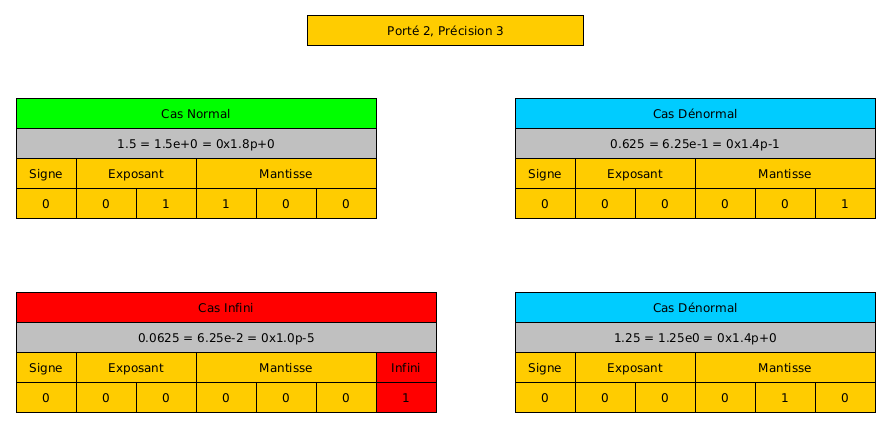
\includegraphics[width=450px]{../ressources/special_case.png}
\caption{\label{fig:org7e5d64a}Rappel des cas spéciaux}
\end{figure}

\label{org2d4bfc0}
\begin{figure}[htbp]
\centering
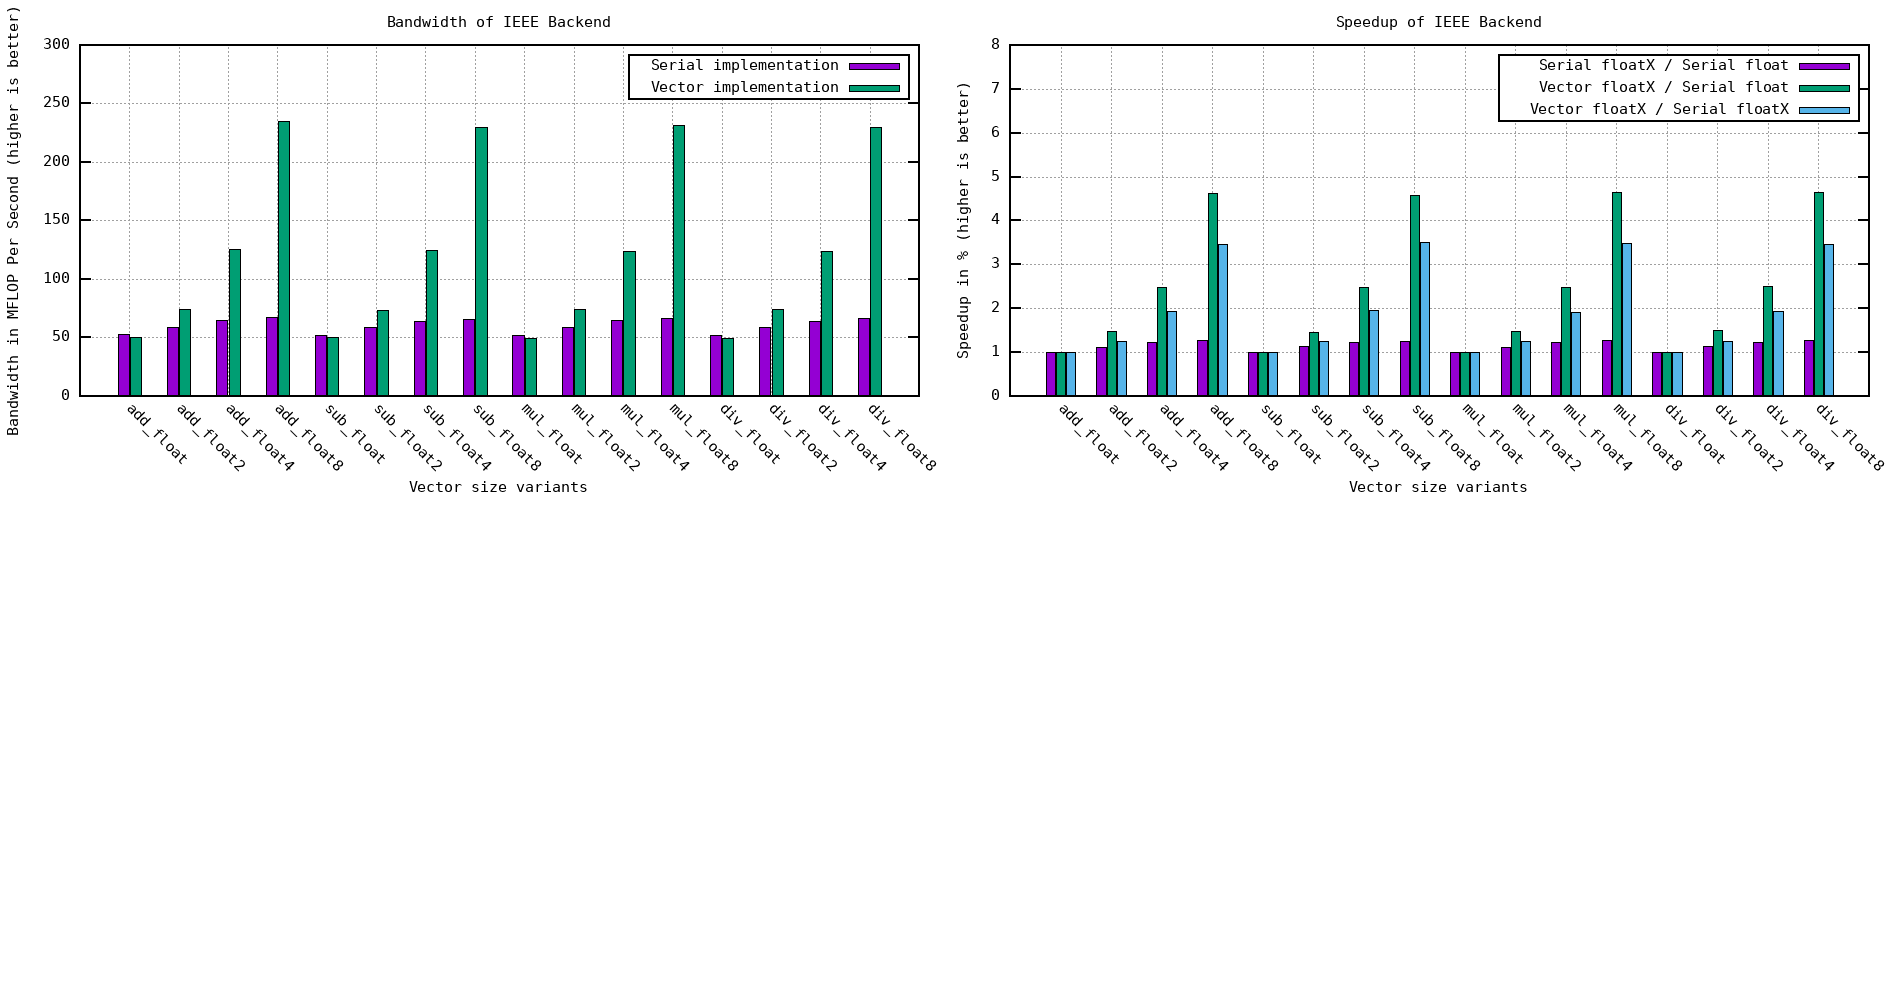
\includegraphics[width=450px]{../ressources/vm_ieee.png}
\caption{\label{fig:org84116da}Résultat du backend IEEE}
\end{figure}

\label{org307795b}
\begin{figure}[htbp]
\centering
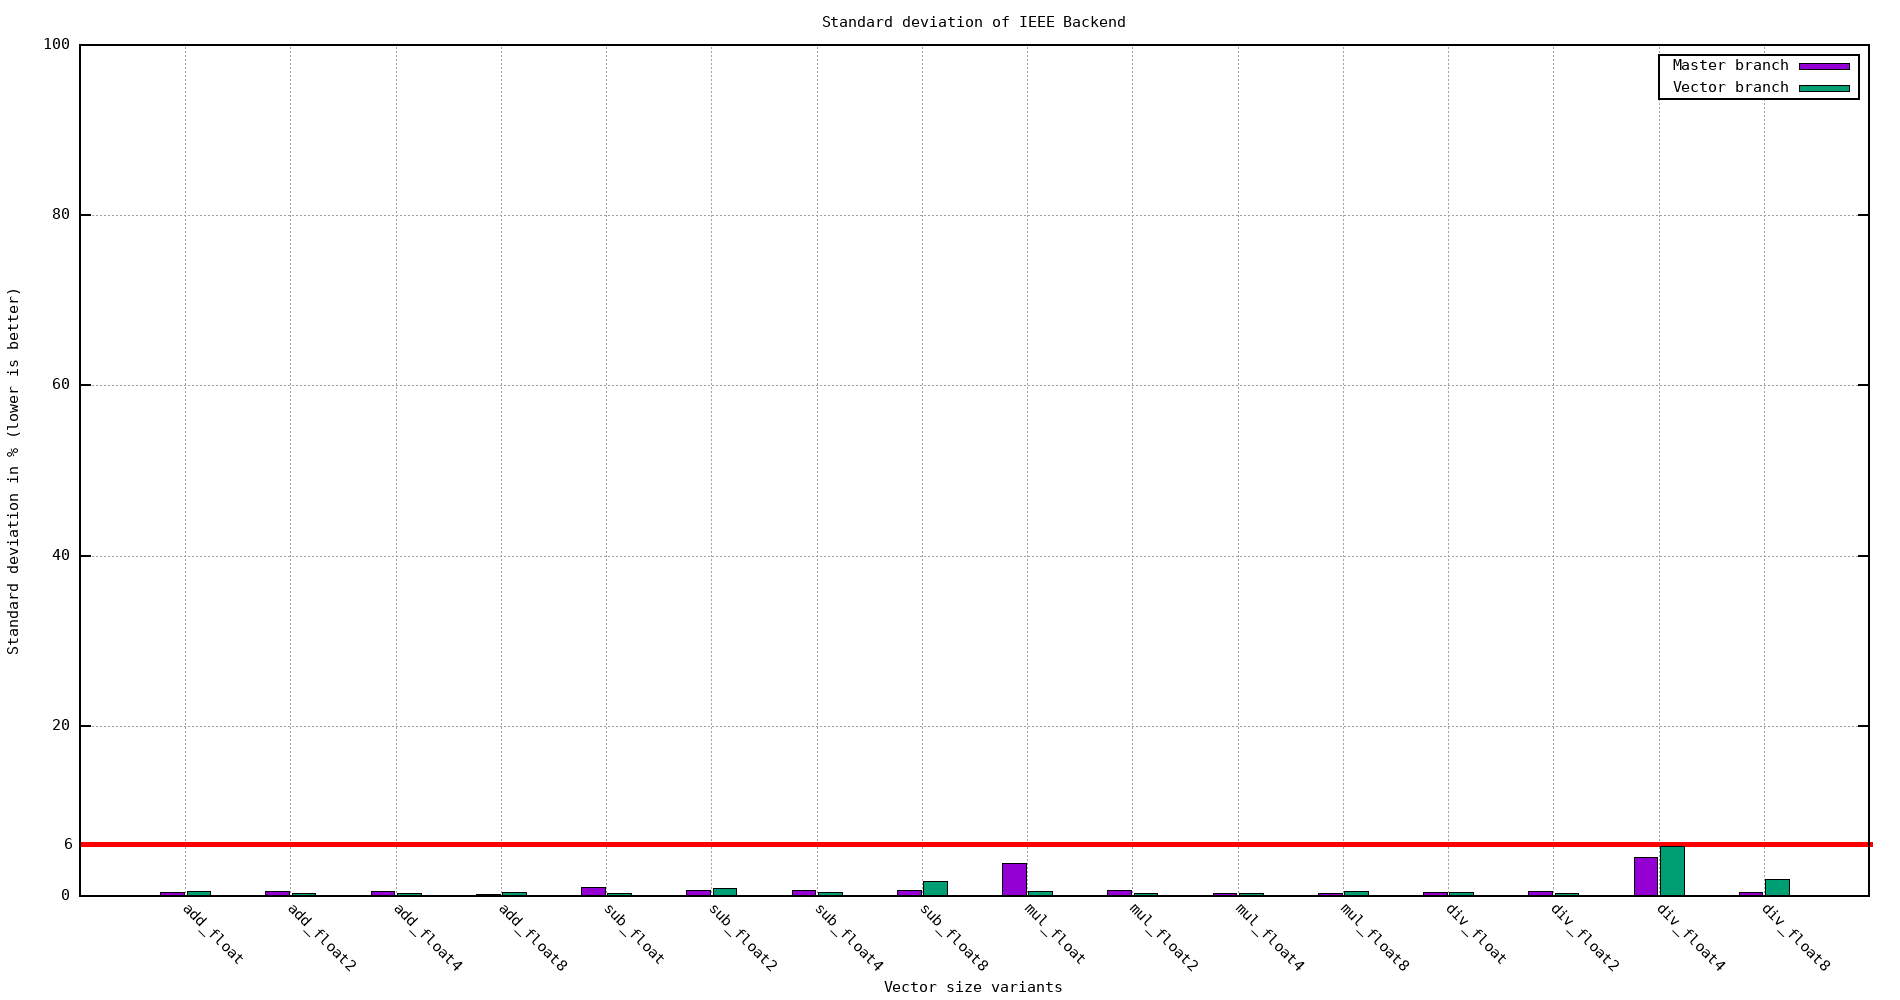
\includegraphics[width=450px]{../ressources/vm_ieee_stddev.png}
\caption{\label{fig:org73ee624}Ecart type du backend IEEE}
\end{figure}

\label{org46bc9dd}
\begin{figure}[htbp]
\centering
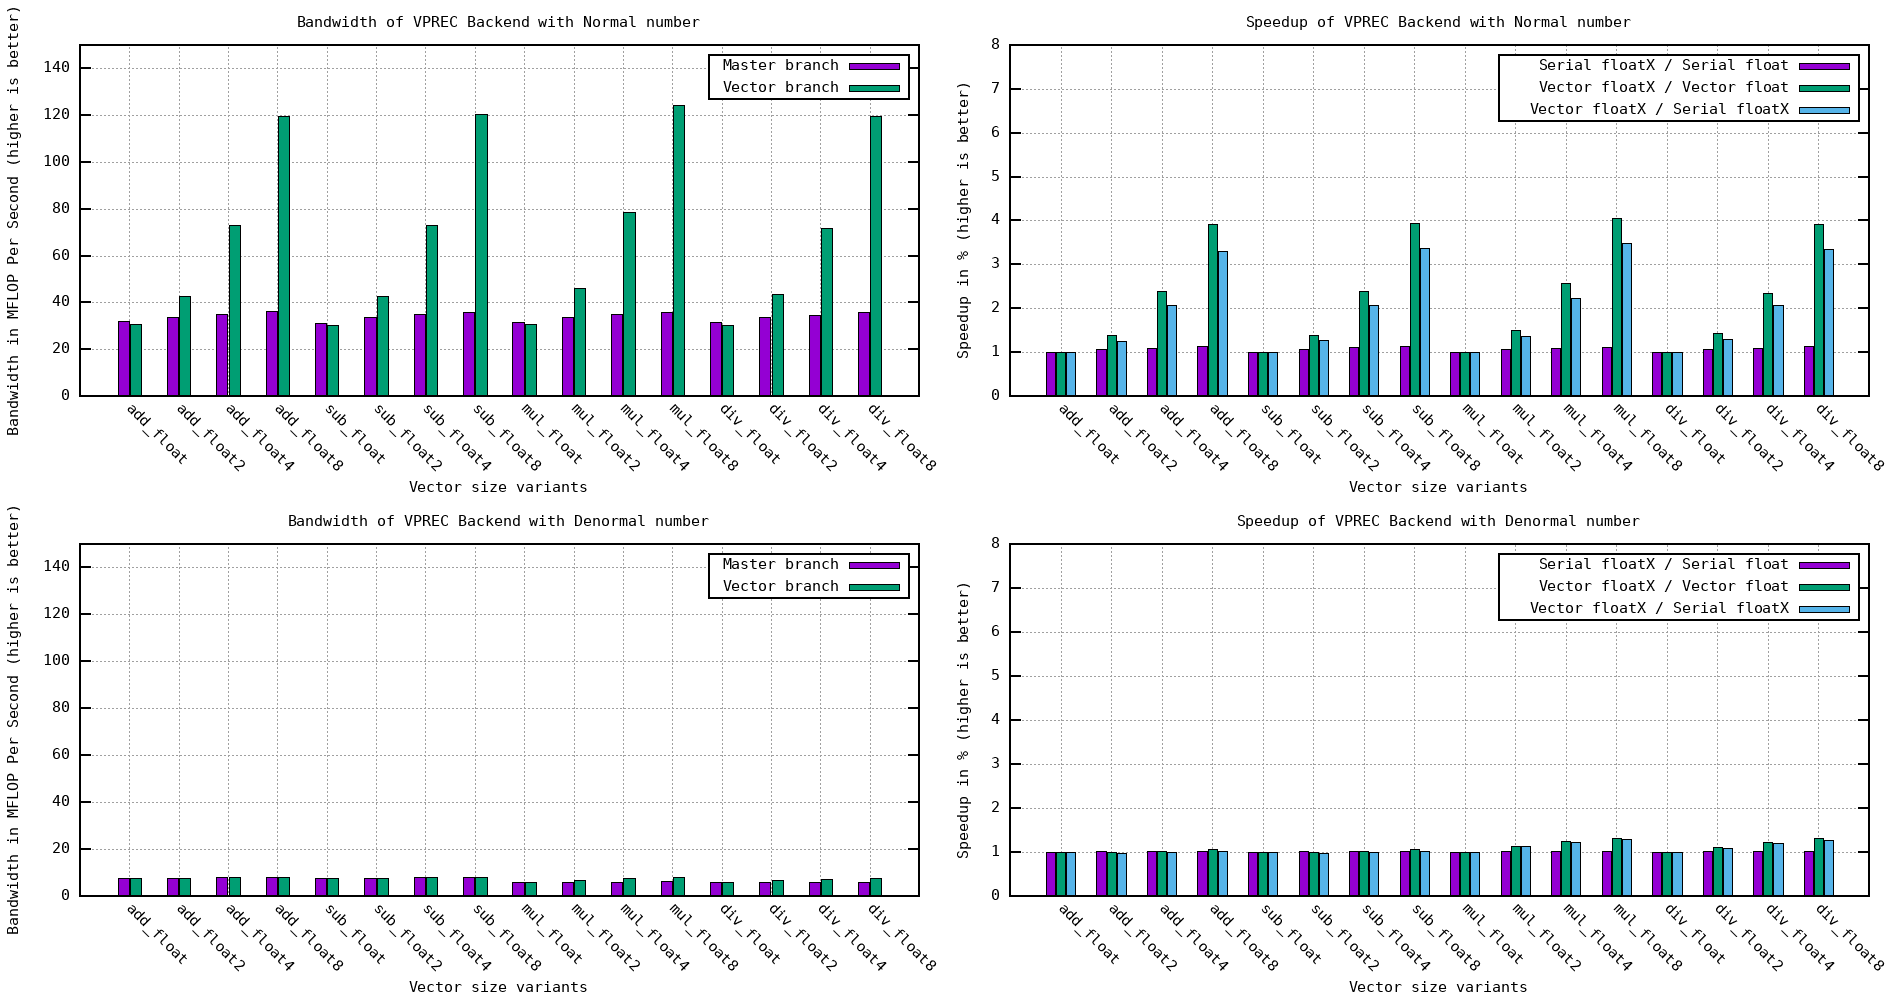
\includegraphics[width=450px]{../ressources/vm_vprec.png}
\caption{\label{fig:org6c49f49}Résultat du backend VPREC}
\end{figure}

\label{org045e625}
\begin{figure}[htbp]
\centering
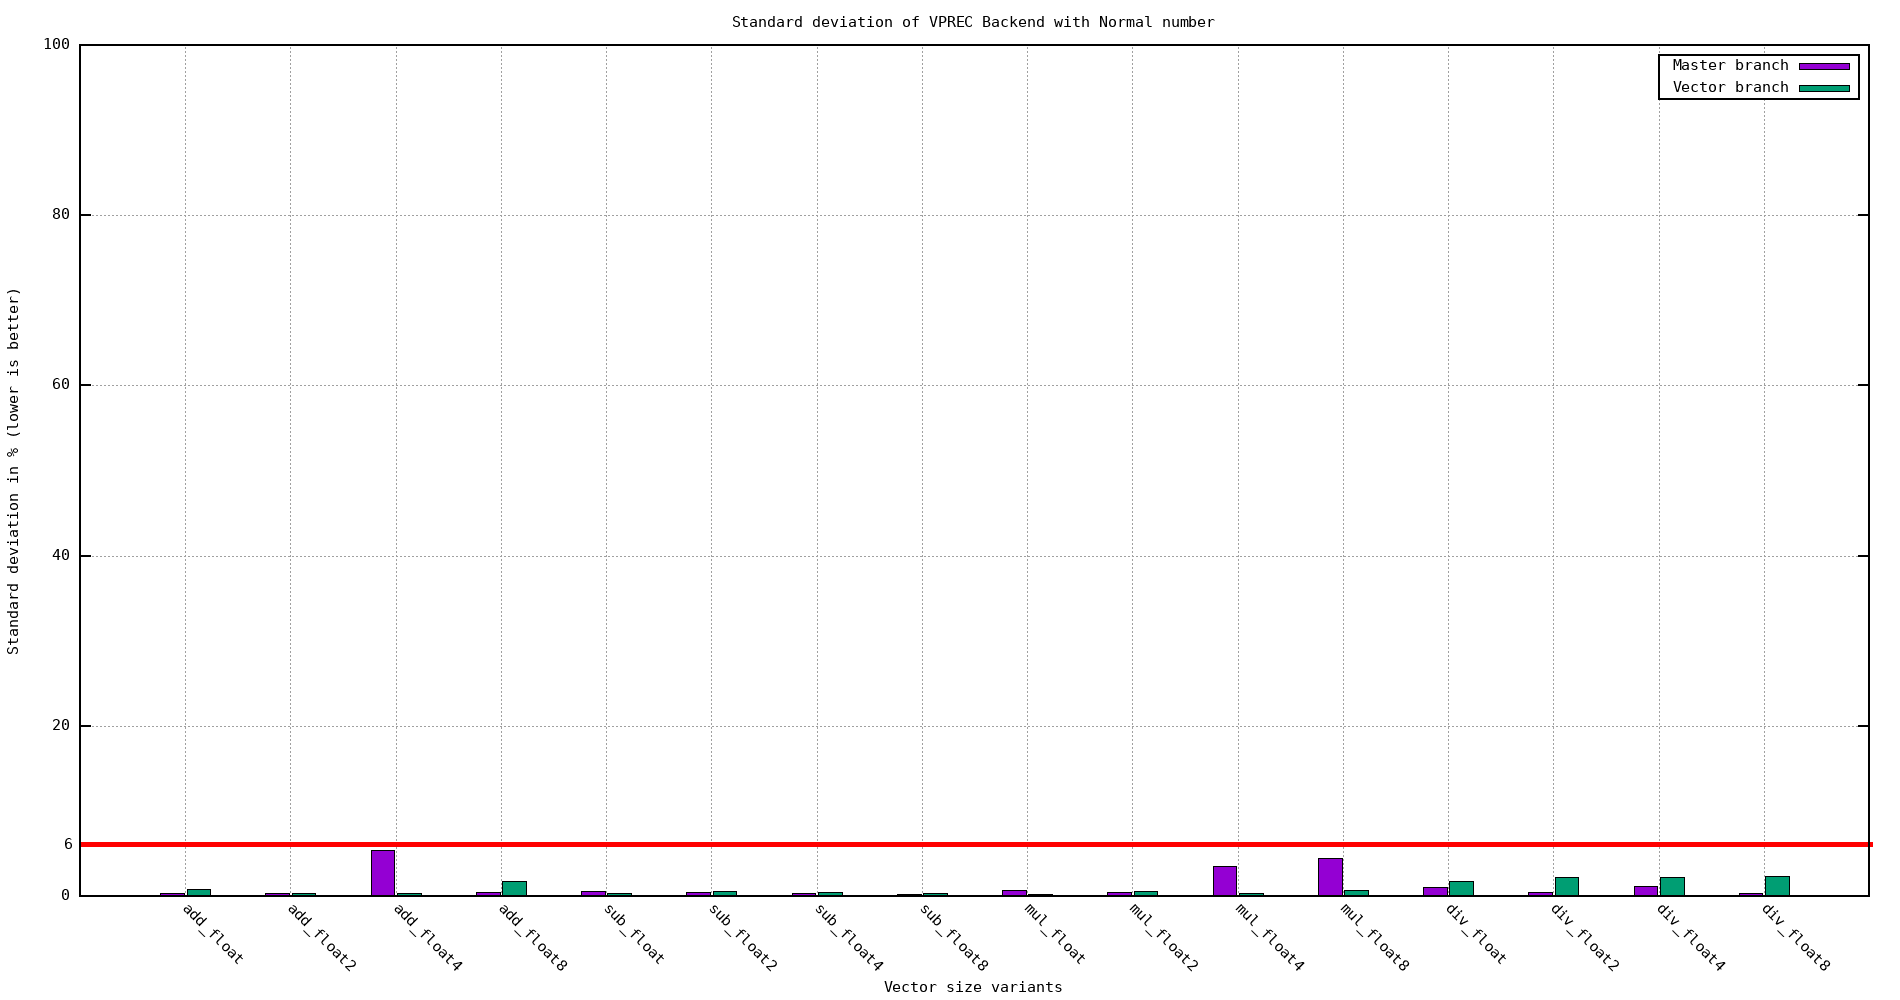
\includegraphics[width=450px]{../ressources/vm_vprec_normal_stddev.png}
\caption{\label{fig:orgc6deb19}Ecart type du backend VPREC avec des nombres normaux}
\end{figure}

\label{org42c2a54}
\begin{figure}[htbp]
\centering
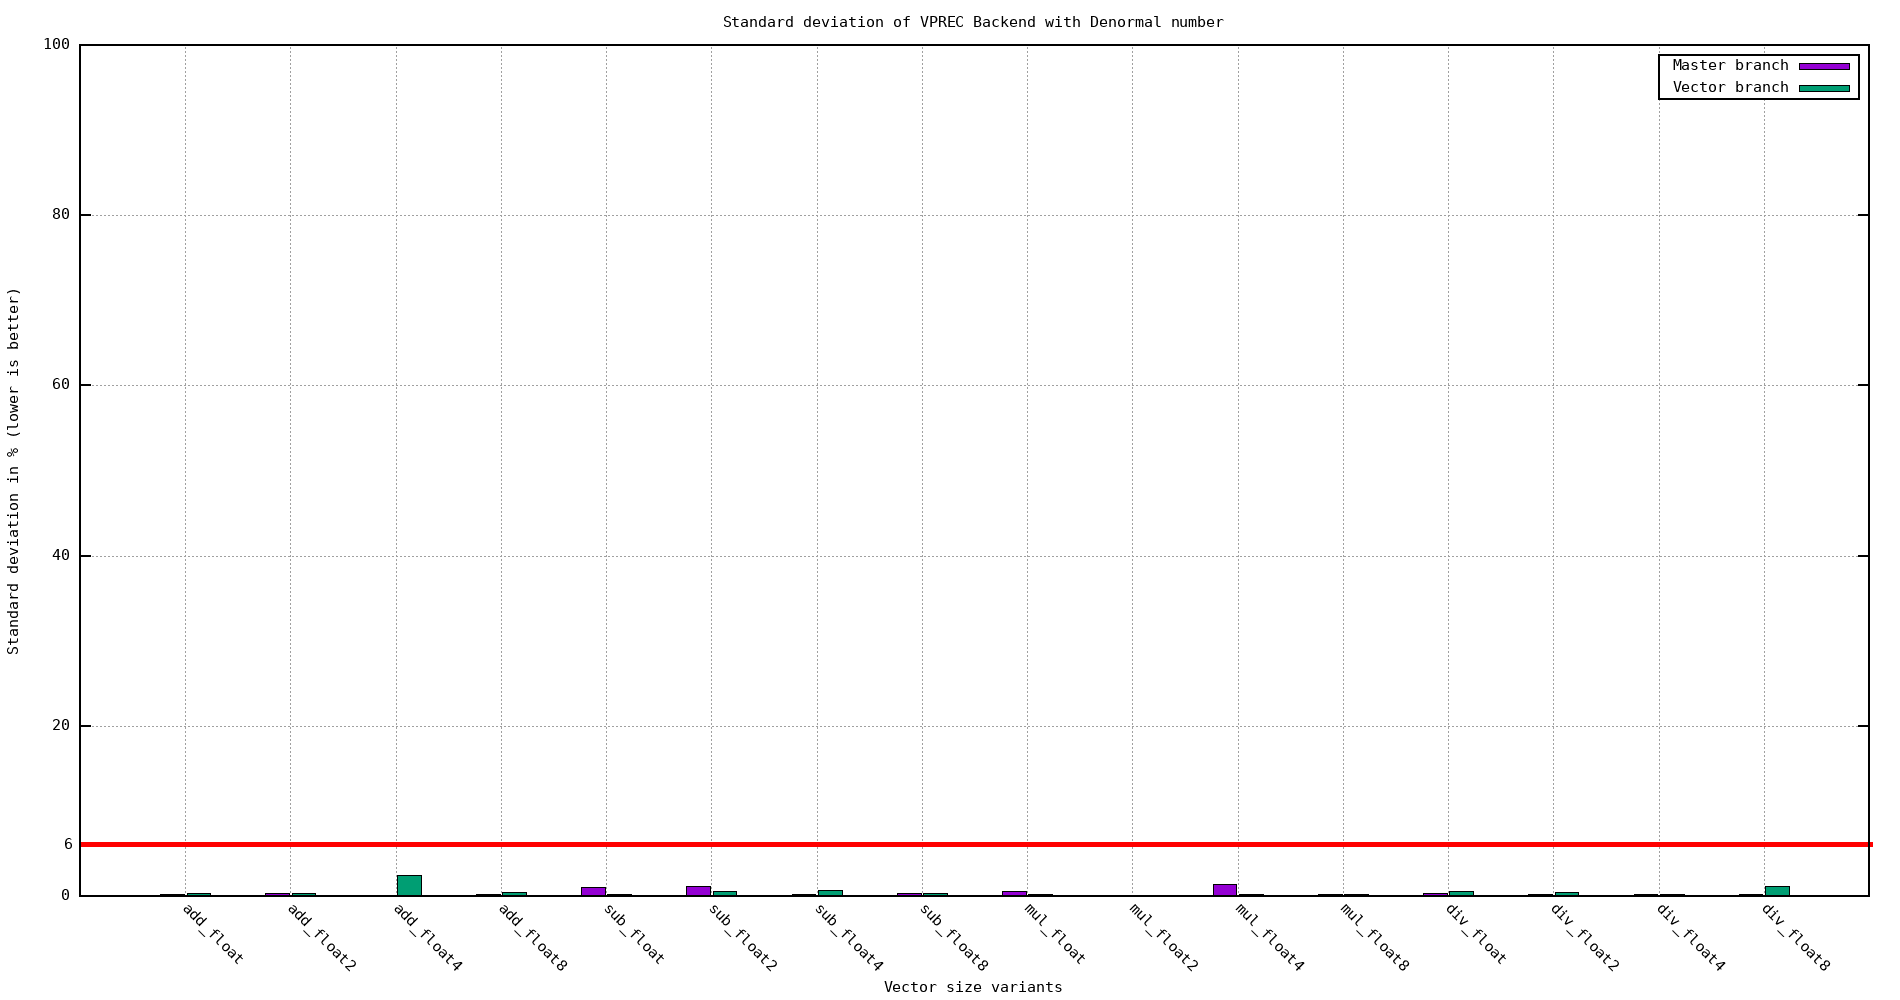
\includegraphics[width=450px]{../ressources/vm_vprec_denormal_stddev.png}
\caption{\label{fig:orgf5d0688}Ecart type du backend VPREC avec des nombres dénormaux}
\end{figure}

\label{org91783ed}
\begin{figure}[htbp]
\centering
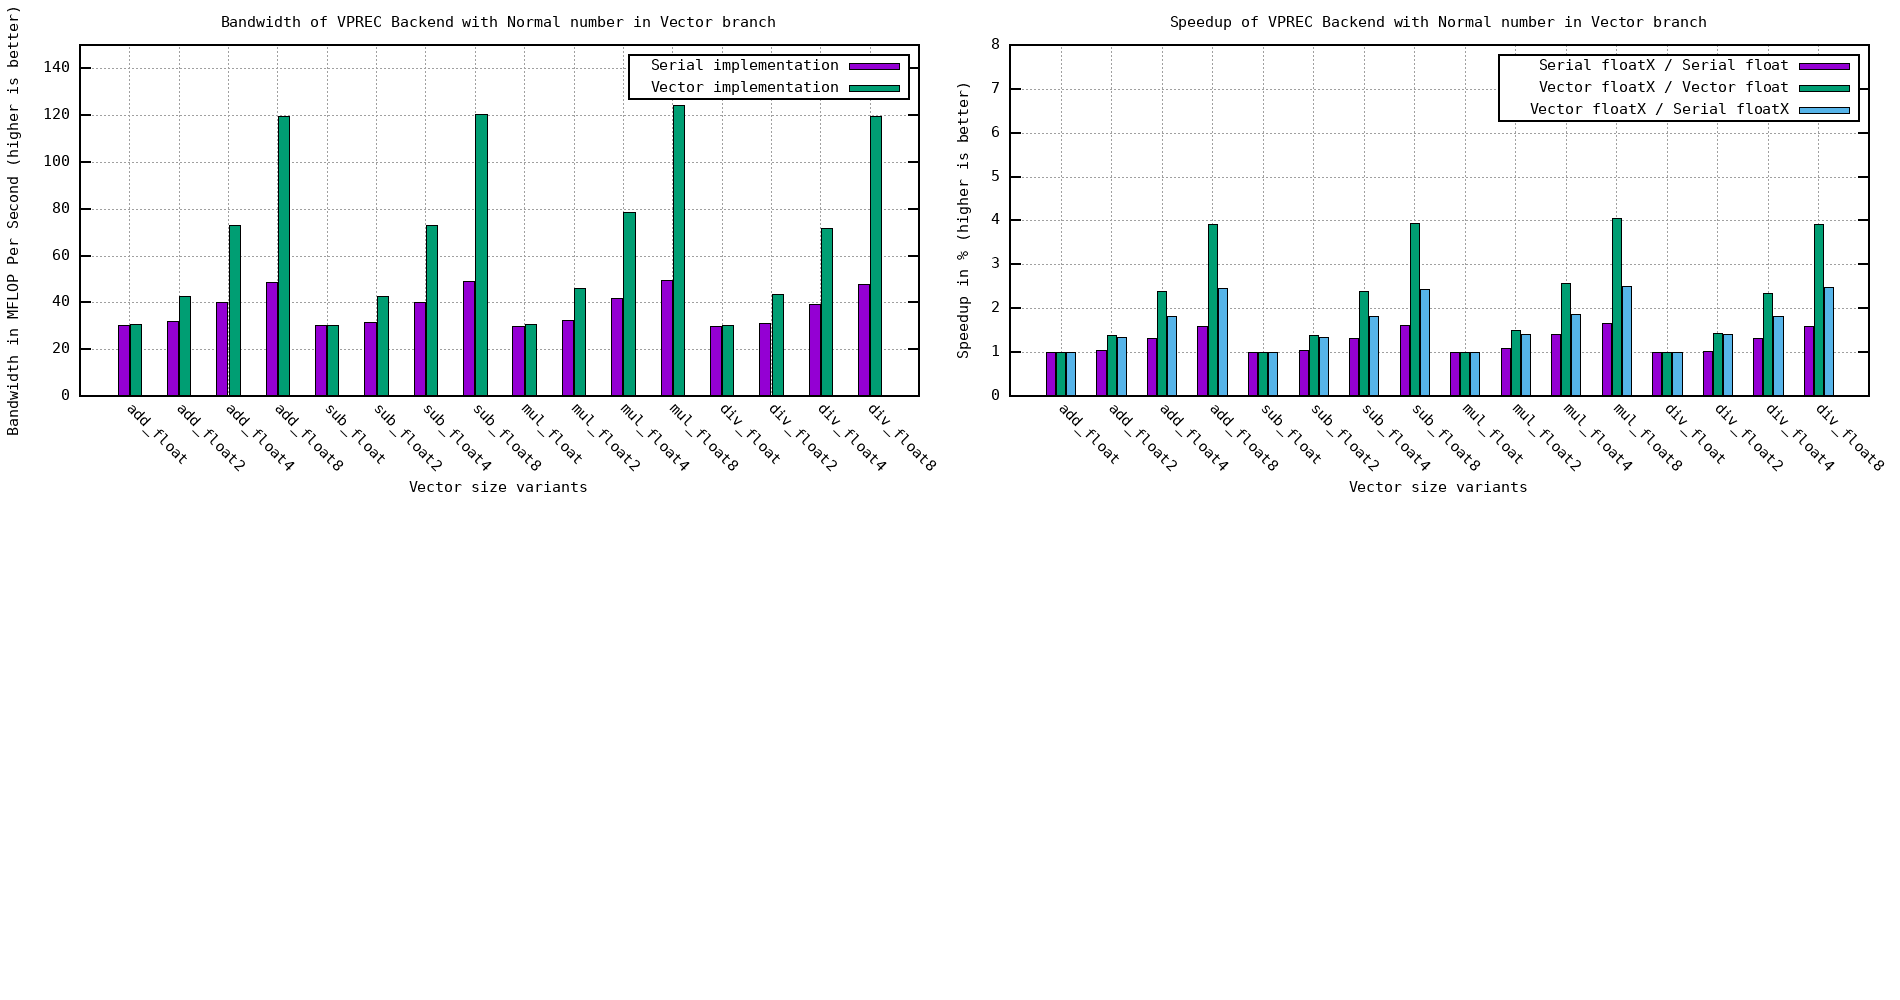
\includegraphics[width=450px]{../ressources/vm_vprec_serial_vs_vector.png}
\caption{\label{fig:org1298293}Résultat du backend VPREC entre l'implémentation sérial et l'implémentation vectorielle des nombres normaux}
\end{figure}

\label{org6e99874}
\begin{figure}[htbp]
\centering
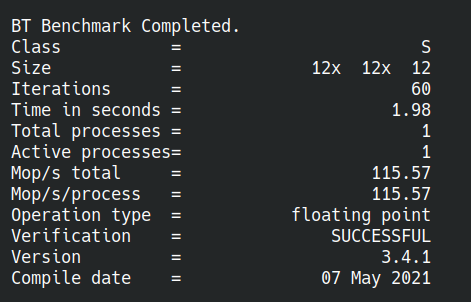
\includegraphics[width=450px]{../ressources/btcompleted.png}
\caption{\label{fig:org12023dc}Rappel des cas spéciaux}
\end{figure}

\label{orged7d9d3}
\begin{figure}[htbp]
\centering
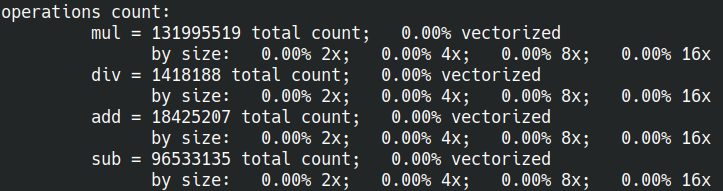
\includegraphics[width=450px]{../ressources/vect1.png}
\caption{\label{fig:orgdd7c55a}Vectorisation au niveau du benckmark BT}
\end{figure}

\label{org7a56fc0}
\begin{figure}[htbp]
\centering
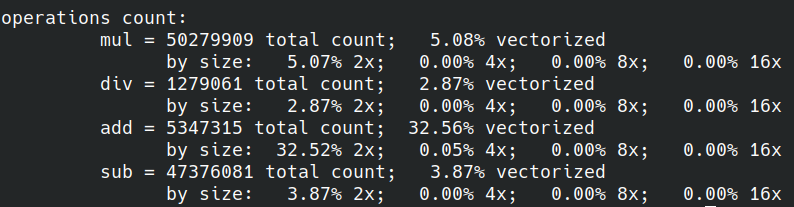
\includegraphics[width=450px]{../ressources/vcopenmp.png}
\caption{\label{fig:org85e30bb}Vectorisation au niveau du benckmark BT}
\end{figure}
\end{document}
